\subsubsection{Convergencia de PageRank}
\label{subsec:exp3}
\begin{LaTeXdescription}
    \item[Objetivo] Estudiar como se comporta la convergencia en funci\'on de
        el factor de navegaci\'on $\alpha$.\\

    \item[Proposici\'on] PageRank propone una soluci\'on donde se observa a un
        conjunto de p\'aginas web como un grafo dirigido. Luego pasa este modelo
        a uno  matem\'atico, utilizando una matriz para computar una soluci\'on.
        Esta matriz, por construcci\'on, termina representando a un grafo
        completo (el grafo original no necesariamente lo era), y los valores del
        mismo dependen principalmente de 2 variables: $\epsilon$ y $\alpha$
        (algoritmo \ref{alg:power_method2}, p\'agina \pageref{alg:power_method2}
        y ecuaci\'on \ref{eq:M_def}, p\'agina \pageref{eq:M_def}). Si se observa
        el algoritmo, se ver\'a que claramente modificar el $\epsilon$ tendr\'a
        como resultado hacer que cada corrida converja en m\'as o menos
        iteraciones, ya que el criterio de parada depende de \'el. As\'i pues,
        no vemos como algo rico experimentar con este valor. En cambio, $\alpha$
        es una variable que modifica en gran medida a nuestra matriz $M$, con lo
        cual es dificil saber cual ser\'a su injerencia en la convergencia (en
        principio). El objetivo, entonces, es ver como $\alpha$ afecta al
        m\'etodo matem\'atico iterativo de la potencia en cuanto a su
        convergencia.\\

    \item[M\'etodo de Experimentaci\'on] Tomaremos 3 instancias de grafos de
        conectividad de p\'aginas web de tama\~no mediano-grande, obtenidas en
        \url{http://snap.stanford.edu/data/\#web}. Luego, correremos el
        algoritmo de PageRank para $\alpha=0.0$; $0.1$; $0.2$; $\dots$; $0.9$ y
        $\epsilon$ fijo en $0.00001$.\\

    \item[Resultados, an\'alisis y discusi\'on]
\end{LaTeXdescription}

\par En el gráfico \ref{subfig:exp3_comp} se exponen la cantidad de iteraciones
necesarias hasta converger a medida que el parámetro $\alpha$ crece. Para las 3
instancias el comportamiento observado es el mismo: a medida que el par\'ametro
$\alpha$ aumenta, la cantidad de iteraciones necesarias para converger crece
exponencialmente. Puede observarse que aunque con valores numéricos diferentes,
las curvas pertenecen a la misma familia de funciones, y por lo tanto tienen un
comportamiento id\'entico (emp\'iricamente hablando) en cuanto a la cantidad de
iteraciones en funci\'on de $\alpha$.

\begin{figure}[H]
    \centering
    \subfloat[][\shortstack{Iteraciones hasta Converger en funci\'on de $\alpha$
            \\Escala Lineal}]{
        \label{subfig:exp3_comp}
        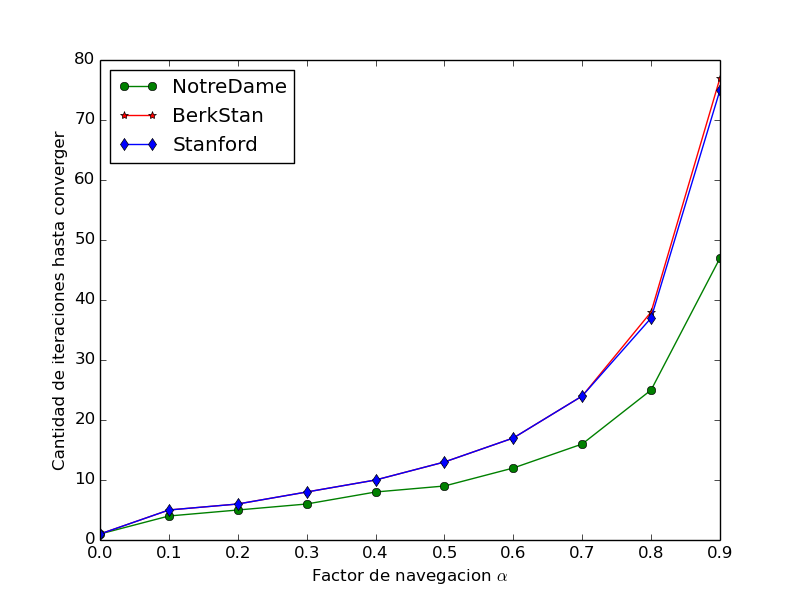
\includegraphics[width=.5\textwidth]{exp3_iteraciones_funcion_alpha.png}
    }
    \subfloat[][\shortstack{Velocidad de convergencia en funci\'on de $\alpha$
            \\Escala logar\'itmica}]{
        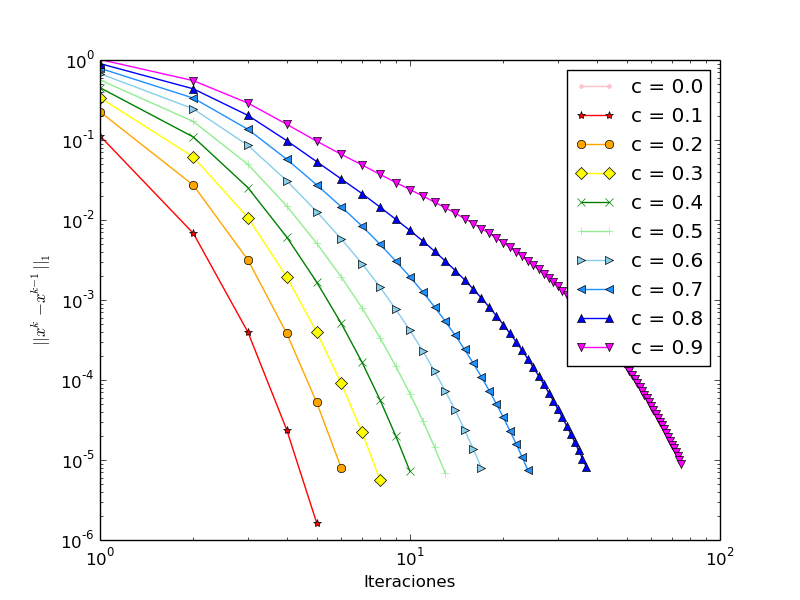
\includegraphics[width=.5\textwidth]{exp3_diff_funcion_iteraciones_standford.png}
        \label{subfig:exp3_diff}
    }
    \caption{An\'alisis de Convergencia en funci\'on de $\alpha$}
\end{figure}

\par Como se explic\'o en la secci\'on \ref{sec:introduccion}, el factor
$\alpha$ hace variar la proporci\'on entre $S$ y la matriz equiprobable a la
hora de definir a $M$. Es decir, en el rango de posibles valores de $\alpha$, la
\'unica manera en la que se afecta a $M$ es en los valores de cada uno de sus
elementos. Pero para ning\'un $\alpha$ se puede pasar a tener un elemento nulo
en $M$ (justamente se quer\'ia tener la representaci\'on de un digrafo
completo). As\'i pues, la pregunta pasa a ser: ¿Por qu\'e a mayor $\alpha$ se
necesitan m\'as iteraciones para converger?

\par Se nos ocurre que, volviendo al contexto de una cadena de Markov y el
navegante aleatorio, un $\alpha$ peque\~no nos genera una matriz de transici\'on
''m\'as'' equiprobable (recordar la definici\'on de $M$ en la ecuaci\'on
\ref{eq:M_def}, p\'agina \pageref{eq:M_def}) y dado que el método de la potencia
comienza inicialmente con el vector equiprobable, le toma pocas iteraciones
converger. A medida que $\alpha$ aumenta, el grafo generado denota más la
navegación estricta por los links entre los sitios, reduciendo la probabilidad
de teletransportación. Es decir, a mayor $\alpha$, el grafo se ''parece m\'as''
al grafo de conectividad original no adulterado (con los dangling nodes ya
resueltos), en el sentido de que $S$ predomina mucho m\'as en $M$ que
$(\rfrac{1}{n})ee^T$. Esta matriz $S$ no necesariamente representa un grafo
fuertemente conexo, una de las condiciones necesarias para asegurar convergencia
del método de la potencia en el contexto de este problema, con lo cual el método
de la potencia inicia sus iteraciones con una, si se quiere, \textbf{seguridad
de convergencia más débil}.

\par Respecto a la velocidad de convergencia, exponemos los resultados de una
sola instancia ya que para las 3 instancias los resultados son similares. Como
puede observarse en el gráfico \ref{subfig:exp3_diff}, a medida que el factor de
navegacion $\alpha$ crece, la velocidad de convergencia disminuye,
obteni\'endose curvas cada vez m\'as pronunciadas.

\par La ''velocidad de convergencia'' la definimos como la distancia
\emph{Manhattan} entre los autovectores $\vec{x^{(k)}}$ y $\vec{x^{(k-1)}}$
calculados en dos iteraciones consecutivas. Mientras mayor sea la distancia,
m\'as r\'apido decimos que se converge\footnote{Asumiendo que $\vec{x^{(k)}} <
\vec{x^{(k-1)}}$, caso contrario nos estar\'iamos alejando del criterio de corte
del m\'etodo, es decir, de converger.}, pues se est\'a acerc\'andose cada vez
\textbf{m\'as rápido} al umbral de corte del algoritmo (basado en $\epsilon$ o
una cantidad fija m\'axima de iteraciones\footnote{Esto se implementa, ya que si
bien la teor\'ia nos indica que el m\'etodo convergir\'a, los errores
n\'umericos de la aritm\'etica finita puede hacer que esto no ocurra.}).

\par Nuestra explicaci\'on para este comportamiento es exactamente la misma que
se expuso para el caso de las iteraciones hasta converger en funci\'on de
$\alpha$. Sin ir m\'as lejos, estamos hablando del mismo fen\'omeno, salvo que
en el caso de la figura \ref{subfig:exp3_diff} hacemos hincapi\'e en
\textbf{como} se acerca el m\'etodo al vector soluci\'on, mientras que en la figura
\ref{subfig:exp3_comp} observamos m\'as en detalle la \textbf{cantidad de
iteraciones} que se necesitan. Sin embargo, ambos gr\'aficos nos muestran lo
mismo: \textit{a qué velocidad}, o \textit{cuánto tiempo/iteraciones} se
requieren para converger en funci\'on de $\alpha$.

\par Ahora bien, hemos visto como $\alpha$ afecta a la convergencia. Si esto
fuera lo \'unico, claramente siempre elegir\'iamos el valor que nos permita
converger m\'as r\'apido. Ocurre que, como vimos en el experimento
\ref{subsec:exp1}, el $\alpha$ afecta al orden obtenido tambi\'en, es decir, a
la calidad del resultado. As\'i pues, la elecci\'on de este par\'ametro ser\'a
la b\'usqueda del equilibrio \emph{efectividad} y \emph{eficiencia}, u entre
calidad del resultado y ti\'empo de c\'omputo (intuitivamente, m\'as iteraciones
implican mayor tiempo de c\'omputo). La bibliograf\'ia consultada nos indica que
en su momento, Google fij\'o inicialmente este par\'ametro en $0.85$,
considerando a este un \emph{trade-off} lo suficientemente
bueno\cite{Bryan2006}\cite{Langville2006}.

\medskip
\par As\'i pues concluimos nuestra experimentaci\'on sobre la convergencia del
m\'etodo de la potencia para PageRank. Llegamos a un resultado inmediato que nos
dice que a mayor $\alpha$ tendremos una velocidad de convergencia menor y, ergo,
una cantidad de iteraciones necesaria mayor para obtener un resultado lo
suficientemente apr\'oximado. Tambi\'en evaluamos brevemente la contracara de
tener un tiempo de convergencia chico: el resultado obtenido no necesariamente
es el mismo ya que predomina m\'as la equiprobabilidad de los ejes de
teletransportaci\'on artificalmente a\~nadidos a la matr\'iz $M$. Tambi\'en
obtuvimos como resultado que este comportamiento es, presumiblemente (har\'ia un
falta un an\'alisis m\'as minucioso para poder afirmarlo), el mismo para
cualquier instancia de entrada, m\'as all\'a de que la cantidad de iteraciones
absoluta entre dos instancias pueda variar para el mismo $\alpha$, el
comportamiento en funci\'on de $\alpha$ parecer\'ia ser el mismo.
